%******************************************************************************************************
%******************************* Fourth Chapter *******************************************************
%******************************************************************************************************

\externaldocument{{../Chapter1/chapter1}}
\externaldocument{{../Chapter2/chapter2}}
\externaldocument{{../Chapter3/chapter3}}
\externaldocument{{../Chapter5/chapter5}}

% **************************** Define Graphics Path **************************
\graphicspath{{Chapter4/Figs/}}


%******************************************************************************************************
%******************************************************************************************************
\chapter{Task Two: Path Following}
\label{task2}

This is the second of two tasks carried out in this project. Whilst our previous task was aimed at planning paths on the ground prior to flight, this task is aimed at commanding the UAV to fly such paths.


%******************************************************************************************************
%******************************************************************************************************
\section{Path Following - Aims}
\label{task2:aims}

The overarching aim for this task is to implement changes to ArduPlane to allow us to fly an air relative Dubins path as defined by the work already completed. Thanks to our path planning solution the UAV does not need to be aware of its ground relative location in order to successfully navigate to our desired point. The path following solution must simply interpret our description of a Dubins path and perform the desired manoeuvres. 

We need to be able to take a mission plan created using MissionPlanner or APM Planner 2 and insert a series of flight commands that will result in the UAV flying our desired Dubins path. To do this, we need to define the these commands in a format the autopulot will understand, and then enable the autopilot to respond to these input commands. 

We can summarise this tasks as being aimed at achieving the following:

\begin{itemize}
	\item Being able to describe a Dubins path using MAVLink messages %TODO introduce mavlink messages
	\item Enabling the UAV to interpret and act upon the new MAVLink messages
	\item Successfully command the UAV to fly a Dubins path, both with and without the presence of wind
	\item Successfully commanding the UAV to fly in wind to a ground relative point using a Dubins path 
\end{itemize}

%TODO finalise aims

%******************************************************************************************************
%******************************************************************************************************
\section{Path Following - Design and Planning}
\label{task2:design}

As with our previous task, we considered our overall aims and split them up into a number of stages. By splitting the task into stages we simplify design, implementation, and testing, whilst also providing clear milestones and cut off points to work well with the planning processes used in this project. These stages were defined as:

\begin{enumerate}
	\item Define the format of new commands required to fly a Dubins path
	\item Enable the UAV to interpret newly added commands
	\item Command the UAV to fly a Dubins path in a no-wind scenario
	\item Command the UAV to fly a Dubins path in the presence of wind
\end{enumerate}

\subsection{Stage 1: Defining New Flight Commands}
\label{task2:design:stage1}

ArduPilot products use MAVLink messages to define all of the commands that may be included in a mission plan; a full list of the current MAVLink messages can be seen at \cite{MavlinkMessages}. A complete mission plan will simply be a collection of MAVLink messages, where each line corresponds to one MAVLink message, consisting of the following fields:

\begin{itemize}
	\item INDEX - an identifier for each command
	\item CURRENT WP - indicating which waypoint the command relates to (irrelevant for this project)
	\item COORD FRAME - indicates whether altitude values are relative to the takeoff altitude or to previous waypoint altitude
	\item COMMAND - the command number used to identify each instruction in the mission plan
	\item PARAM1 - optional parameter field
	\item PARAM2 - optional parameter field
	\item PARAM3 - optional parameter field
	\item PARAM4 - optional parameter field
	\item PARAM5/X/LONGITUDE - optional parameter field or a GPS longitude value 
	\item PARAM6/Y/LATITUDE - optional parameter field or a GPS latitude value
	\item PARAM7/Z/ALTITUDE - optional parameter field or an altitude value
	\item AUTOCONTINUE - flag to indicate whether to continue through the mission plan after this command
\end{itemize}

 To keep our system as simple as possible, it was decided that the easiest way to describe a Dubins path using MAVLink messages was to generate an individual message for each segment of the path. This would allow us to create a MAVLink message that indicated whether the segment needed to be a left-hand turn, right-hand turn, or a straight line. The console application created for path planning accepts the UAV's airspeed as an inpurt argument, and outputs the path as three segments and displays their length. This meant that it was very simple to create a MAVLink message indicating just two things; the segment turn direction, and the duration for the UAV to fly it. 

 As our paths had been designed independent of GPS co-ordinates, each MAVLink message only needed to include the command value, and the duration value in one of the parameter fields. We didn't need any GPS or altitude information in PARAM5, PARAM6, or PARAM7. By following the information found in the developer's wiki at \cite{ArduPilotMAVLink}, we were able to add four new commands. As we knew that our new commands were to be navigation commands, we followed the MAVLink convention of starting the names with ``MAV\_CMD\_NAV\_''. We decided to name our new messages as follows:

 \begin{enumerate}
 	\item MAV\_CMD\_NAV\_DUBIN\_LEFT
 	\item MAV\_CMD\_NAV\_DUBIN\_RIGHT
 	\item MAV\_CMD\_NAV\_DUBIN\_STRAIGHT
 	\item MAV\_CMD\_NAV\_DUMMY\_WP
 \end{enumerate}

 The last command was a dummy command, included so that we would be able to include one of these commands into a simulation, print out a message into the simulator console and therefore be confident that our commands were being read correctly by the autopilot. As the name would suggest, this final command was never intended to do anything other than provide a verification technique.

 The new message types were defined in \path{.../ardupilot/libraries/GCS\_MAVLINK/message\_definitions/ardupilotmega.xml}. This is the file where developers add platform specific commands, not intended to be shared with other ArduPilot products such as ArduCopter; this is because GCS\_MAVLINK is a shared library, in which most MAVLink messages are defined in the file \path{.../ardupilot/libraries/GCS\_MAVLINK/message\_definitions/common.xml}.

 An example of one of these definitions is as follows:

 \begin{minipage}{\linewidth}
\begin{lstlisting}[language=XML]
<entry name="MAV_CMD_NAV_DUBIN_RIGHT" value="86">
	<description>Perform a RIGHT turn segment of a dubins path turn</description>
	<param index="1">Duration of time to fly this segment</param>
	<param index="2">Empty</param>
	<param index="3">Empty</param>
	<param index="4">Empty</param>
	<param index="5">Empty</param>
	<param index="6">Empty</param>
	<param index="7">Empty</param>
</entry>
\end{lstlisting}
\end{minipage}

The numerical value chosen for each command is very important, as we have to ensure that all MAV\_CMD\_NAV entries are below 95, which is the value of the MAV\_CMD\_NAV\_LAST command, whilst also ensuring we are using values not currently in use. After double checking their values, the value 84 was assigned to the dummy command, 85 to the left hand turn command, 86 to a right hand turn command, and 87 to a straight segment. By running the \textit{generate.sh} script in the GCS\_MAVLINK directory we finalised this stage of the task, inserting our new commands into the header files used by ArduPlane to interpret MAVLink messages.


\subsection{Stage 2: Using New Flight Commands}
\label{task2:design:stage2}

The next stage of this work was to enable the autopilot to recognise our new commands, and in the case of the Dubins turn commands, to store the time parameter we had passed it. 

\subsection{Stage 3: Flying a Dubins Path in the Absence of Wind}
\label{task2:design:stage3}

\subsection{Stage 4: Flying a Dubins Path in the Presence of Wind}
\label{task2:design:stage4}

%******************************************************************************************************
%******************************************************************************************************
\section{Path Following - Implementation}
\label{task2:implementation}

\subsection{Stage 1: Defining New Flight Commands}
\label{task2:implementation:stage1}

\subsection{Stage 2: Using New Flight Commands}
\label{task2:implementation:stage2}

\subsection{Stage 3: Flying a Dubins Path in the Absence of Wind}
\label{task2:implementation:stage3}

\subsection{Stage 4: Flying a Dubins Path in the Presence of Wind}
\label{task2:implementation:stage4}

\begin{figure}[htbp!] 
\centering    
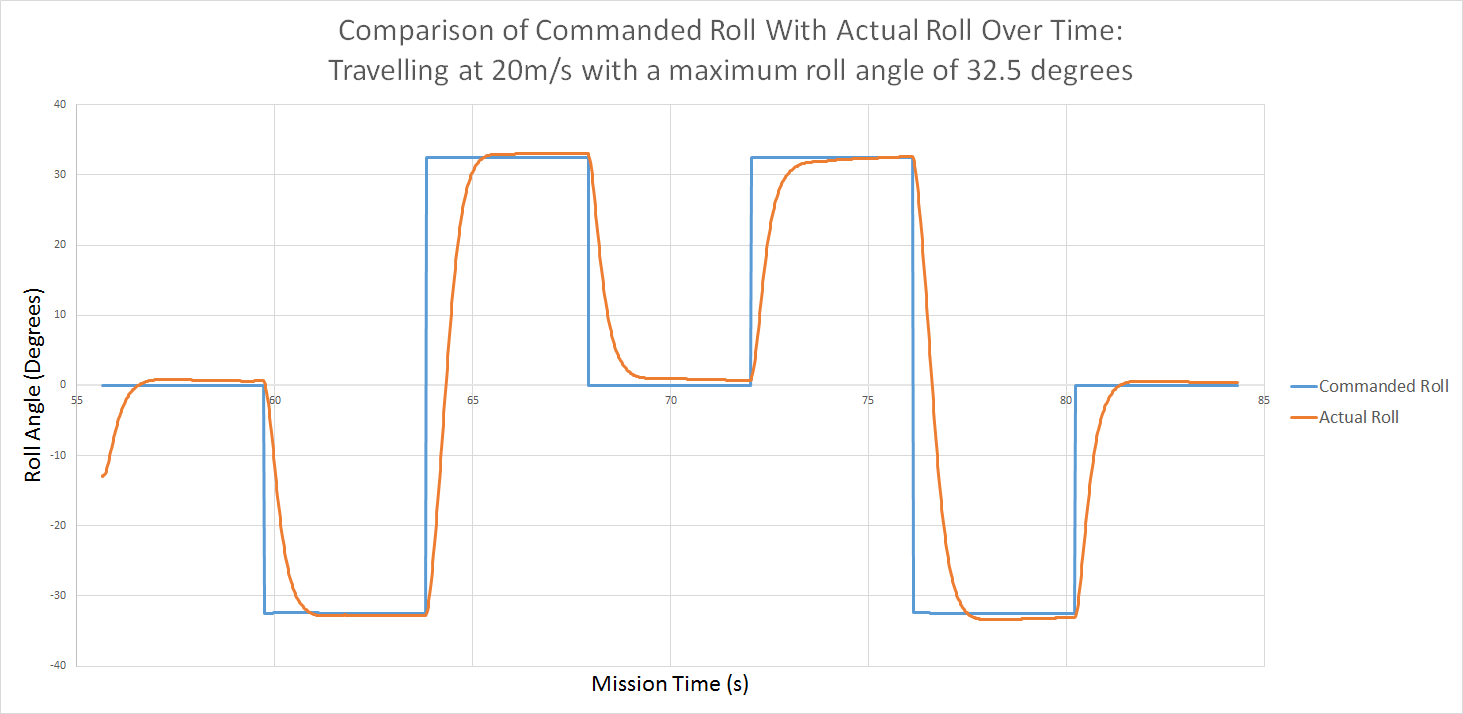
\includegraphics[angle=90,origin=c,height=0.7\textheight]{32_20_RollComparison}
\caption[]{roll comparison}
\label{fig:32rollcomparison}
\end{figure}


%******************************************************************************************************
%******************************************************************************************************
\section{Path Following - Testing}
\label{task2:testing}

The testing and verification techniques available are quite limited with regards to this task. By utilising the JSBSim based flight simulator we are able to simulate the flight of a given UAV over a mission we supply to it. After this, we can use the MAVExplorer utility to analyse the log files and to plot out a map with a trace of the UAVs flightpath compared to its mission.

\subsection{Stage 1: Defining New Flight Commands}
\label{task2:testing:stage1}

\subsection{Stage 2: Using New Flight Commands}
\label{task2:testing:stage2}

\subsection{Stage 3: Flying a Dubins Path in the Absence of Wind}
\label{task2:testing:stage3}

\subsection{Stage 4: Flying a Dubins Path in the Presence of Wind}
\label{task2:testing:stage4}



1	0	3	85	2000	0	0	0	0	0	0	1
2	0	3	87	2000	0	0	0	0	0	0	1
3	0	3	85	2000	0	0	0	0	0	0	1
